\chapter{Introduction}
\thispagestyle{chapterBeginStyle}

\section{Thermalization in closed systems}
From all of the long-standing problems that have bothered physicists, the relationship
between micro and macro world is perhaps one of the most disputed ones. On the one
hand, we have a remarkably successful theory of statistical mechanics and the seemingly
irreversible laws of thermodynamics~\autocite{huang1987statistical,feynman1998statistical}.
On the other hand, we have a no less successful theory of quantum mechanics,
which predicts the reversibility of microscopic dynamics~\autocite{landau1991quantum,Sakurai2017}.
One can then pose a question, when and why a far-from equilibrium isolated quantum system
can be accurately described using equilibrium statistical mechanics?

\paragraph{Eigenstate Thermalization Hypothesis}It was already suggested by John von Neumann in 1929 that a proper way of
thinking about thermalization of quantum systems is by looking at physical
observables instead of wave functions or density matrices of the whole system~\autocite{Neumann192930}.
Following the review article by~\textcite{DAlessio2016}, we say that an 
observable undergoes thermalization if it evolves with time towards the
prediction of microcanonical ensemble and stays in the vicinity of it for majority
of future times. The question is, what is necessary for this thermalization to happen?
To answer it, let us imagine that we have an isolated quantum system in a pure
state \(\ket{\psi_{\textrm{initial}}}\). We want to investigate evolution
of some observable \(O\) under time-independent Hamiltonian \(H\) with
eigenstates \(\ket{n}\) and corresponding energies \(E_n\). Writing the time-dependent
wave function as \(\ket{\psi(t)}=\sum_{n} C_{n} \mathrm{e}^{-i E_{n} t}\ket{n}\),
 \(C_n =  \braket{n}{\psi_{\textrm{initial}}}\), we have 
\begin{align}
    O(t) & =\matrixel{\psi(t)}{O}{\psi(t)}=\sum_{m, n} C_{m}^{*} C_{n} 
    \mathrm{e}^{i\left(E_{m}-E_{n}\right) t} O_{m n} \nonumber\\
    &=\sum_{n}\abs{C_{n}}^{2} O_{nn}+\sum_{n \neq m} C_{m}^{*} C_{n} 
    \mathrm{e}^{i\left(E_{m}-E_{n}\right) t} O_{m n}\label{eq:time evolution}
\end{align}
We immediately see that, assuming lack of degeneracy, long-time average of the off-diagonal
part must be equal to zero and what remains is the diagonal part.
This is a prediction of the so-called \textit{diagonal ensemble}~\autocite{Cassidy2011}.
It basically means that the system `remembers' its initial conditions via the constant
coefficients \(\abs{C_n}^2\). At first, it is not clear how we could reach the prediction of 
microcanonical ensemble. Moreover, the time necessary for the second term to vanish 
in many-body systems could easily exceed the age of our universe~\autocite{DAlessio2016}.
Nevertheless, such thermal relaxation was observed in experiments with isolated
cold atomic gasses~\autocite{Rigol2012,Rigol2008854,Hung2010,Kinoshita2006,Hofferberth2007}.

This is where an insight from Random Matrix Theory (RMT), pioneered by~\textcite{Wigner1955}
in context of nuclear physics, comes into play. He observed that if we were to write
a Hamiltonian in a generic and not fine-tuned basis, it would essentially be a random matrix
(subject to symmetry constraints). It can then be shown within RMT formalism~\autocite{mehta2004random},
that matrix elements of an Hermitian operator \(O\) in eigenbasis of a random Hamiltonian 
can be written as
\begin{equation}
    O_{mn} \approx \bar{O}\delta_{mn} + \sqrt{\frac{\overline{O^2}}{\dimension}}R_{mn}
    \label{eq:RMT}
\end{equation}
where \(\bar{O} = \frac{1}{\dimension}\sum_i O_i\), \(O = \sum_i O_i \ketbra{i}{i}\), \(\dimension\)
it the dimension of underlying Hilbert space and \(R_{mn}\) is either real or complex (depending on symmetries of the Hamiltonian) random
variable with zero mean and unit variance. Using equation~\eqref{eq:RMT}, we can then 
disentangle the prediction of diagonal ensemble from the initial conditions
\begin{equation}
    \sum_{n}\abs{C_n}^2 A_{nn} \approx \bar{A}\sum_{n}\abs{C_n}^2 = \bar{A}
\end{equation}
obtaining a results consistent with microcanonical ensemble, albeit without energy dependence
so equivalent to the infinite-temperature limit. Furthermore, off-diagonal elements are exponentially
small in system size, so it is enough to eliminate phase coherence between matrix elements with
largest contribution to the expected value, for the second term in equation~\eqref{eq:time evolution}
to vanish. This can happen on much shorter timescales that would be required for eliminating
phase coherence between all eigenstates~\autocite{DAlessio2016}.

Nonetheless it is not yet enough, as RMT misses two crucial points in order to be able to relate
it to real systems. First, the expectation values should depend on energy and second, relaxation
times should be observable dependent. These shortcomings were fixed in groundbreaking works
of~\textcite{Deutsch19912046,Srednicki1994} giving rise to the \textit{Eigenstate Thermalization Hypothesis} (ETH)
It is often stated in form of an \textit{ansatz} for matrix elements of observables expressed in
eigenbasis of a Hamiltonian~\autocite{Srednicki1999}
\begin{equation}
    O_{mn} = O(\bar{E}) \delta_{mn} + \mathrm{e}^{S(\bar{E})/2}f_{O}(\bar{E},\omega)R_{mn}
    \label{eq:ETH}
\end{equation}
where \(\bar{E} = (E_n+E_m)/2\), \(\omega=E_n-E_m\) and \(S(\bar{E})\) is the thermodynamic
entropy an energy \(\bar{E}\). Both \(O(\bar{E})\) and \(f_{O}(\bar{E},\omega)\) are smooth
functions of their parameters and \(O(\bar{E})\) is equivalent to the expected value in microcanonical
ensemble. Finally, as in RMT, \(R_{mn}\) is a random real or complex variable. At the moment it is
unknown in general whether the ETH holds for a given observable in a given system,
however it is expected to be valid for all physical observables~\autocite{DAlessio2016}. 
Numerical clues for the validity of ETH have been found in many strongly correlated lattice models
for example hard core bosons, interacting spin chains~\autocite{Santos2010,Rigol2010,Khatami2013,Rigol2009a},
and fermions~\autocite{Neuenhahn2012,Rigol2009}. For more details on ETH see
the review by~\textcite{DAlessio2016}, on which this Introduction is based.


\paragraph{Generalized Gibbs Ensemble}In a generic system exhibiting ETH, after thermalization the expectation values
of observables can be calculated using density matrix from relevant Gibbs ensembles
(because of equivalence of ensembles one can use either microcanonical, canonical or
grand canonical one).
For example in the grand canonical ensemble \(\hat{\rho} \propto \mathrm{e}^{(H-\mu N)/kT}\)
and \(\bar{O}\approx \tr(O \hat{\rho})\).
However, there exists a class of models, called \textit{integrable}\footnote{A very brief review of integrability is presented in Appendix~\ref{app:int}.},
for which the ETH does not hold. There is no widely accepted definition of quantum
integrability, but for our purpose it will be enough to characterize such systems by
existence of an extensive number of (quasi-)local operators \(\set{\hat{I}_k}\) that commute with
the Hamiltonian and with each  other\footnote{For relevant definitions see Section~\ref{sec:prelim}.}.
Just as in classical mechanics existence of integrals of motion imposes an constraint on phase
space available to a system, the lack of thermalization in integrable quantum systems can be
attributed to the existence of extensive number of conservation laws, instead of only a few like
in nonintegrable ones (such as energy or momentum). Remarkably, it was shown by~\textcite{Rigol2007}
that the usual approach employed in statistical mechanics, namely maximizing many-body entropy
\(S = k_B \tr(-\hat{\rho}\ln(\hat{\rho}))\) subject to constraints yields a very successful result.
It is now know as the Generalized Gibbs Ensemble (GGE)
\begin{equation}
    \hat{\rho}_{\mathrm{GGE}} = \frac{\exp({-\sum_k \lambda_k I_k})}{
        \tr[\exp({-\sum_k \lambda_k I_k})]}  
\end{equation}
where \(I_k\) are the integrals of motion and \(\lambda_k\) are Lagrange multipliers fixed
by requiring that \(\tr(\hat{\rho}_{\mathrm{GGE}}I_k) = \langle I_k\rangle(t=0)\).
In generic nonintegrable models where the only integrals of motion are the Hamiltonian and
particle number operator, GGE reduces to the usual grand canonical ensemble. 
Many numerical test have been carried out suggesting that integrable system, in general, do not
relax to thermal equilibrium and that GGE accurately describes properties of few-body
 observables after thermalization~\autocite{Cassidy2011,Rigol2007,Vidmar2016,Cazalilla2006}.
Nonetheless, finding agreement with predictions from thermal equilibrium does not necessarily
mean that the model is nonintegrable, as there are fine-tuned states that relax towards
predictions of thermal equilibrium despite integrability of underlying 
system~\autocite{Rigol2012,Rigol2011a,He2012}. 

\section{Motivation and the aim of this dissertation}
As ETH is anticipated to be valid in generic
nonintegrable systems, so is GGE likely to describe thermalization in generic integrable system.
However, on the contrary to nonintegrable models, classification of appropriate 
conserved quantities in integrable models is in general a difficult task~\autocite{DAlessio2016}.
This problem will be our main interest in Chapter~\ref{chap:iom}, where 
following~\textcite{Mierzejewski2015a} we will describe in detail an algorithm allowing for
systematic classification of all conserved quantities in a system given by a tight-binding
Hamiltonian. As further motivation for the search of integrals of motion, in
Chapter~\ref{chap:iom} we will also introduce the well-known concept of Mazur 
bound~\autocite{Mazur1969,Suzuki1971} and a rather new phenomenological tool for studying
quantum many-body systems --- integrated spectral function~\autocite{Vidmar2021}. 
As an application of introduced methodology, we will study the energy current and
two \textit{noncommuting} conserved quantities in paradigmatic spin-\(1/2\) XXZ model.


Complete integrability is not a common property in the quantum world.
Many system requires fine-tuning of their parameters to achieve this, with perhaps a single
exception given by systems exhibiting many-body localization. Furthermore, we usually
do not have precise enough control over real-world systems to perform such fine tuning,
so full integrability is rarely seen (albeit some signatures of it were 
observed in an experiment~\autocite{Khemani2019}). It is thus desirable to investigate
\emph{almost} integrable system, where the integrability-breaking perturbation is small.
In classical systems, the solution to this problem lies within the KAM theorem, however
no such conclusive result exists in the quantum world (for details see Appendix~\ref{app:int}).
In such weakly perturbed quantum system the number of conserved quantities must be nonextensive,
so at least some of them must decay. Investigating long-time behavior of autocorrelation functions of
aforementioned energy current and two noncommuting observables 
in spin-(1/2) XXZ model will be the subject of Chapter~\ref{chap:decay}. In case of
the titular noncommuting integrals of motion we report a novel
result about linear scaling of relaxation time with perturbation strength and Gaussian,
instead of the expected exponential~\autocite{mallayya2019}, decay of relevant autocorrelation functions.
 
The remainder of this chapter will be devoted to a short introduction
to the Heisenberg model and its modification, namely the titular XXZ model.

\section{Heisenberg model of magnetism\label{sec:XXZ}}
    It is well known, that we can divide magnetic materials into two broad groups: those which
exhibit magnetic properties in reaction to external magnetic field and those which have a nonzero
magnetic moment without external field~\autocite{spalek2015}. First group consists of paramagnetic
and diamagnetic systems. In the former, nonzero net magnetic moment comes from alignment of
valence electrons' spins in the direction of external magnetic field. In the latter, we deal with
 an inductive effect in which external field induces magnetic dipoles opposing the field that have
induced them. Diamagnetism exists in all materials, however it is usually much weaker than other magnetism related
effects and thus only detectable in the absence of them. Second group includes ferromagnets, which
exhibit spontaneous magnetization below Curie temperature, and ferrimagnets, which are 
composed of two ferromagnetic sublattices with different spontaneous magnetization. There
are also antiferromagnets, which are essentially a special case of ferrimagnets in which the two sublattices,
below the so-called N{\'e}el temperature, have spontaneous magnetizations of equal magnitude
but opposite directions~\autocite{nolting2018theoretical}.

There are two paradigmatic models of magnetism, namely the Heisenberg model, which describes magnetism
of localized electrons and their magnetic moments (spins), and the Hubbard model which deals with
magnetism of delocalized electrons, called the itinerant magnetism. 
In this chapter we will deal with the former of two models.
First, a physics-motivated derivation of Heisenberg model will be presented. Afterwards,
on our way to XXZ model, we will discuss the mathematical details and various modifications
of original model. Our review of this topic will be based on the books by~\textcite{spalek2015} and 
thesis by~\textcite{Ng2011HeisenbergM}.

\subsection{Heisenberg-Dirac exchange interaction}
\paragraph{Coulomb interaction}The story begins with two electrons interacting with each other via Coulomb potential.
An electron can be described by two quantities, its position in space and its spin.
Two facilitate these two degrees of freedom, we say that \(i\)-th electron's wave function
lives in a Hilbert space which is a tensor product of spacial 
wave functions' space and spin wave functions' space, i.e.\ \(\mathcal{H}_i \cong L^2(\RR^3)
\otimes \mathfrak{h}_i \), where \(L^2(\RR^3)\) is the usual space of square-integrable functions on
\(\RR^3\), and \(\mathfrak{h}_i \cong \CC^2\) is a two-dimensional vector space spanned by
\(\ket{\ua} = \binom{1}{0} \) and \(\ket{\da} = \binom{0}{1}\).
The combined wave function of a composite two-particle system it then an element of
\(\mathcal{H}_1 \otimes \mathcal{H}_2\), which can be decomposed into spacial and spin
components, i.e\ \(\mathcal{H}_1 \otimes \mathcal{H}_2 \cong\mathcal{H}_{\mathrm{space}} 
\otimes \mathcal{H}_{\mathrm{spin}}\), where \(\mathcal{H}_{\mathrm{space}} 
\cong L^2(\RR^3) \otimes L^2(\RR^3)\) and \(\mathcal{H}_{\mathrm{spin}} \cong
\mathfrak{h}_1 \otimes \mathfrak{h}_2\). 

Hamiltonian of two interacting electrons is given by
\begin{equation}
    H_C = \underbrace{-\frac{\hbar^2}{2m} \laplacian_1  
    -\frac{\hbar^2}{2m} \laplacian_2 }_{\textrm{free particles}}
     + \underbrace{V(\bm{r}_1,\bm{r}_2)}_{\textrm{interaction}}
     \label{eq:Coulomb Hamiltonian}
\end{equation}
where in case of Coulomb interaction we have \(V(\bm{r}_1,\bm{r}_2)=\frac{\mathrm{e}^2}
{\abs{\bm{r}_1-\bm{r}_2}}\).
Formally, this Hamiltonian acts on the space \(\mathcal{H}_1 \otimes \mathcal{H}_2\).
However, it depends only on the spatial coordinates \(\bm{r}_1,\bm{r}_2\) and not on
the spin coordinates, so essentially
its actions is restricted to the \(\hspac\) part of the full Hilbert space.
This is a crucial observation that lead to the development of Heisenberg model. We will now
seek a way to replace this Hamiltonian by an equivalent one acting only on 
\(\hspi\).

\paragraph{Two-electron wave function}It is time to invoke the Pauli exclusion principle, which requires the composite wave function
of two electrons to be antisymmetric under exchange of pairs of coordinates (both spatial and
spin degrees of freedoms are treated like coordinates). Because 
Hamiltonian~\ref{eq:Coulomb Hamiltonian} does not depend explicitly on spin, the total
wave function \(\psi\) can be expressed as tensor product \(\psi_{\mathrm{space}} 
\otimes \psi_{\mathrm{spin}} \). Antisymmetric nature of \(\psi\) then requires one 
of these components to be antisymmetric \((a)\) and the other to be symmetric \((s)\). 
Spatial wave functions (unnormalized) are of the form
\begin{align}
    &\spas = \psi_1(\bm{r}_1)\otimes \psi_2(\bm{r}_2) +
    \psi_2(\bm{r}_1)\otimes \psi_1(\bm{r}_2) \\
    &\spaa = \psi_1(\bm{r}_1)\otimes \psi_2(\bm{r}_2) -
    \psi_2(\bm{r}_1)\otimes \psi_1(\bm{r}_2)
\end{align}
where \(\psi_1,\psi_2 \in L^2(\RR^3)\). Spin wave functions are elements of \(\CC^2 \otimes \CC^2\)
and are given by
\begin{align}
    &\spis = \ket{\ua\ua},\; 
    \ket{\ua\da} + \ket{\da\ua},\; \ket{\da\da} \\
    &\spia = \ket{\ua\da}-\ket{\da\ua}
\end{align}
where \(\ket{\ua\ua}\) is an usual shorthand notation for \(\ket{\ua}_1 \otimes
\ket{\ua}_2\). Moreover, symmetric spin wave functions
constitute a triplet state, whereas antisymmetric one is a singlet state. 

Possible two-electron wave functions are thus either \(\varphi=\spas
\otimes \spia\) or \(\chi = \spaa
\otimes \spis\). Expected value of energy of Coulomb interaction 
in these states is given by
\begin{align}
    &\expectationvalue{H_C}{\varphi} = \expectationvalue{H_C}{\spas} = E^{(s)}\\
    &\expectationvalue{H_C}{\chi} = \expectationvalue{H_C}{\spaa} = E^{(a)} 
\end{align}
Because \(\spas\) is symmetric with respect to \((\bm{r}_1-\bm{r}_2)\),
we have \(E^{(s)}>E^{(a)}\). Therefore, it is energetically
favorable for our system to pick the total wave function that is antisymmetric
in space and symmetric in spin coordinates.

\paragraph{Spin-spin interaction}Under the Coulomb interaction, symmetric and antisymmetric spin wave functions are not
directly distinguished. It is the difference between spatial parts, together with Pauli
exclusion principle that forces the choice of a triplet state. Let us now do something
similar, but the other way around. We can formally recast the Coulomb Hamiltonian as a
spin-spin interaction acting on \(\hspi\) that would distinguish
between symmetric and antisymmetric spin wave functions and thus fix the spatial part.
Let \(\tau^x,\tau^y,\tau^z\) be the \(2\cross 2\) Pauli matrices
\begin{equation}
\tau^x = \mqty(\pmat{1}),\;\;\;\tau^y = \mqty(\pmat{2}),\;\;\;\tau^z= \mqty(\pmat{3})
\label{eq:Pauli matrices}
\end{equation}
Together with a \(2\cross 2\) identity matrix \(\Id\) they form a basis of vector space of
Hermitian operators acting on a single spin Hilbert space.
They are traceless and of unit determinant. By direct computation it can be checked that
they satisfy a particular commutation and anticommutation relations
\begin{align}
    &\comm{\tau^j}{\tau^k} = 2 i \varepsilon_{jkl}\tau^{l}\\
    &\anticommutator{\tau^j}{\tau^k} = 2 \delta_{jk} \Id_{2\cross 2}
\end{align}
which in turn leads to the following important property
\begin{align}
        \comm{\tau^{j}}{\tau^{k}} + \anticommutator{\tau^{j}}{\tau^{k}} 
    &=\left(\tau^{j} \tau^{k}-\tau^{k} \tau^{j}\right)+\left(\tau^{j} \tau^{k}+\tau^{k} 
    \tau^{j}\right) \nonumber \\
    i \varepsilon_{j k l} \tau^{l}+\delta_{j k} \Id_{2\cross 2} &= \tau^{j} \tau^{k}
\end{align}
We define an operator via a formal dot product
\begin{equation}
    \bm{\tau}_1 \cdot \bm{\tau}_2 = \tau_1^x \otimes \tau_2^x + \tau_1^y \otimes \tau_2^y +
    \tau_1^z \otimes \tau_2^z  
\end{equation}
where subscripts refer to which electron's Hilbert space they act on. 
Let us now examine how this operator acts on \(\ket{\ua\ua}\) spin wave function
\begin{align*}
    \bm{\tau}_1 \cdot \bm{\tau}_2 \ket{\ua\ua} &= 
    \left(\tau_1^x \ket{\ua}_1\right) \otimes \left(\tau^x_2 \ket{\ua}_2\right) + 
    \left(\tau_1^y \ket{\ua}_1\right) \otimes \left(\tau^y_2 \ket{\ua}_2\right) +
    \left(\tau_1^z \ket{\ua}_1\right) \otimes \left(\tau^z_2 \ket{\ua}_2\right)\nonumber\\
    &= \left( \smqty(\pmat{1}) \smqty(1\\0)\right) \otimes \left( \smqty(\pmat{1}) \smqty(1\\0)\right) +
    \left( \smqty(\pmat{2}) \smqty(1\\0)\right) \otimes \left( \smqty(\pmat{2}) \smqty(1\\0)\right)+
    \left( \smqty(\pmat{3}) \smqty(1\\0)\right) \otimes \left( \smqty(\pmat{3}) \smqty(1\\0)\right)\\
    &= \smqty(0\\1) \otimes \smqty(0\\1) + \smqty(0\\i) \otimes \smqty(0\\i) + 
    \smqty(1\\0) \otimes \smqty(1\\0) = \ket{\ua\ua}
\end{align*}
So \(\ket{\ua\ua}\) is an eigenvector of \(\bm{\tau}_1 \cdot \bm{\tau}_2\) with
an eigenvalue \(1\). Carrying out such computations for the three remaining states we get
that all symmetric states are eigenvectors with eigenvalue \(1\), whereas the
antisymmetric state is also an eigenvector, but with eigenvalue \(-3\). 
We could have also obtained this result in a more elegant way by referring directly
to quantum mechanics and algebra of spin angular momentum~\autocite{Sakurai2017}.
If we set \(\hbar = 1\) (which from now on will always be the case), we have the usual
spin vector operators \(\bm{S}_i = \left(\Sx_i,\Sy_i, \Sz_i\right) \) where
 \(S_i^{\alpha} = \tau_i^{\alpha}/2\).
Squares of these operators commute with all other \(S_i^{\alpha}\), hence are the
Casimir operators of their algebras and by Schur's Lemma are proportional to
the identity~\autocite{Woit2017}.
The proportionality constant is equal for spin\(-s\) particles to \(s(s+1)\) and thus
all single spin-\(1/2\) states are eigenvectors of these operators with eigenvalue \(3/4\). 
We can also construct square of total spin angular momentum operator
\(\bm{S}^2 = (\bm{S}_1 + \bm{2}_2)^2\) for which our triplet (total spin \(S=1\)) and singlet
(total spin \(S=0\)) are eigenvectors with eigenvalue \(S(S+1)\). On the other hand, we 
can calculate \(\bm{S}^2\) directly to obtain the following equation
\begin{equation}
    S(S+1)\Id_{2\cross 2} = \bm{S}_1^2 + \bm{S}_2^2 + 2\bm{S}_1\cdot \bm{S}_1 = \frac{3}{2}\Id_{2\cross 2} + 2\bm{S}_1\cdot\bm{S}_2
\end{equation} 
Rearranging it, replacing \(\bm{S}_i\) by \(\bm{\tau}_i/2\) and inserting appropriate values
of \(S\) we recreate the previously obtained result on eigenvalues of 
\(\bm{\tau}_1\cdot\bm{\tau}_2\).

\paragraph{Equivalent Hamiltonian}After this detour into the world of quantum mechanics of spin, let us return to the problem
at hand. We have established that triplet states and singlet state are eigenvectors of 
\(\bm{\tau}_1 \cdot \bm{\tau}_2\) operators with eigenvalues \(1\) and \(-3\) respectively.
Consider now the following Hamiltonian acting on \(\hspi\)
\begin{equation}
    H_S = \frac{3 E^{(a)} + E^{(s)}}{4} + \frac{E^{(a)} - E^{(s)}}{4} \bm{\tau}_1 \cdot \bm{\tau}_2
    \label{eq:Coulomb recasted}
\end{equation}
It is easy to see that eigenvalues of \(H_S\) are \(E^{(a)}\) for symmetric spin states
(corresponding to \(\spaa\)) and \(E^{(s)}\) for antisymmetric spin state (corresponding to \(\spas\)).
We have thus obtained a Hamiltonian that is equivalent to \(H_C\), yet acting on space 
\(\hspi\) rather than \(\hspac\). Setting \(J = E^{(a)} - E^{(s)}\) and ignoring
constant energy offset, we finally arrive at the Dirac-Heisenberg exchange interaction
\begin{equation}
    H_S = \frac{J}{4} \bm{\tau}_1 \cdot \bm{\tau}_2
\end{equation}
or, expressed in terms of usual spin operators
\begin{equation}
    H_S = J \bm{S}_1 \cdot \bm{S}_2
    \label{eq:heisenberg dirac}
\end{equation}
Constant \(J\) is called the exchange integral and its sign determines the nature of system described
by this Hamiltonian. If \(J<0\), then symmetric triplet states have lower energy and we say that
the ground state is ferromagnetic. On the other hand, if \(J>0\) then antisymmetric singlet
state has lower energy and the ground state is antiferromagnetic.  

\subsection{One-dimensional XXZ model}
\paragraph{Heisenberg model}It now straightforward to generalize this exchange interaction to spins living on an arbitrary
lattice, by summing the spin-disguised Coulomb interaction~\eqref{eq:heisenberg dirac} over all pairs
of spins
\begin{equation}
    H = \frac{1}{2}\sum_{i\neq j} J_{ij} \bm{S}_i \cdot \bm{S}_j
    \label{eq:Heisenberg model}
\end{equation}
The factor \(\frac{1}{2}\) is introduced to mitigate double-counting of pairs.
This is the so-called Heisenberg (Heisenberg-Dirac) Hamiltonian. What this Hamiltonian
does is describe correlation between spins of single particles located in atoms \(i\) and \(j\)
(lattice sites), induced by repulsive Coulomb interaction. 
In practical calculations it is often assumed that electrons are well localized, and thus
the value of the exchange integral falls off quickly enough with increasing distance between them
that only the nearest neighbors interactions are important. Moreover, \(J_{ij}\) is also assumed
to be the same between those nearest neighbors
\begin{equation}
    J_{ij} = \begin{cases}
        J,\;\;\; i \textrm{ is a direct neighbor of } j\\
        0,\;\;\; \textrm{otherwise}
    \end{cases}
\end{equation}
These assumptions reduce Heisenberg Hamiltonian to its most popular form
\begin{equation}
    H = -\frac{J}{2}\sum_{\langle i,j \rangle} \bm{S}_i \cdot \bm{S}_j
    \label{eq:canonical Heisenberg}
\end{equation}
where summation index \(\langle i,j \rangle\) indicates that this sum should be performed over all pairs
of nearest neighbors (with repetitions).

\paragraph{One-dimensional lattice}From now on we restrict our attention to the case of one-dimensional lattices and
nearest neighbors interaction. First, let us set up the stage. We are interested in studying
a one-dimensional chain of \(L\) spin-\(1/2\) interacting fermions with periodic boundary conditions,
i.e.\ arranged in a circular ring. For visualization of periodic boundary conditions in 
one and two-dimensional cases see Figure~\ref{fig:pbc}.
The underlying Hilbert space is then a \(2^L\)-dimensional
tensor product of \(L\) single spin spaces \(\hspi = \bigotimes_{j=1}^{L}\mathfrak{h}_j\).
To upgrade a single spin operator \(\sigma\) to this product space we use the
standard embedding~\autocite{Ng2011HeisenbergM}
\begin{equation}
    \sigma_j = \underbrace{\Id_{2\cross 2} \otimes \cdots \otimes \Id_{2\cross 2}}_{j-1}
     \otimes \;\sigma \otimes \Id_{2\cross 2} \otimes \cdots \otimes \Id_{2\cross 2}
    \label{eq:embedding}
\end{equation}
Subscript \(j\) means that even though this operator formally acts on
\(\hspi\), it acts in a nontrivial way only on \(\mathfrak{h}_j\). 

Hamiltonian~\eqref{eq:canonical Heisenberg} in one dimension has the following form
\begin{equation}
    H_{XXX} =  J\sum_{j=1}^L \left( \Sx_{j}\Sx_{j+1} + \Sy_{j}\Sy_{j+1} + \Sz_{j}\Sz_{j+1} \right)
    \label{eq:XXX}
\end{equation}
where periodic boundary conditions are imposed by requiring that \(S^{\alpha}_{L+1} = 
S^{\alpha}_{1}\). 
Sometimes it is also called the isotropic XXX model. A characteristic property of the XXX model
is that is posses \(SU(2)\) symmetry (rotation of spins), which causes
difficulties in numerical studies. Therefore, breaking this symmetry is often desirable.
This can be achieved by introducing anisotropy in form of different exchange integrals for
different directions. Resulting model is known in the literature as the XYZ model
\begin{equation}
    H_{XYZ} = \sum_{j=1}^L  \left( J_{x} \Sx_{j}\Sx_{j+1} + J_{y} 
    \Sy_{j}\Sy_{j+1} + J_{z} \Sz_{j}\Sz_{j+1} \right)
\label{eq:XYZ}
\end{equation}
It is interesting to note, that this is not only a mathematical trick
to simplify numerical calculations, but a system described by this Hamiltonian was realized in
practice~\autocite{Pinheiro2013}.
To reduce the number of parameters, we can single out a particular direction.
We can then choose it to be the \(z\) direction
and set \(J_x = J_y \equiv J \neq J_z \equiv J\Delta\). As a result we get the titular XXZ model
\begin{equation}
    H_{XXZ} = J\sum_{j=1}^L  \left( \Sx_{j}\Sx_{j+1} + \Sy_{j}\Sy_{j+1} \right) + 
    J\Delta \sum_{j=1}^L \Sz_{j}\Sz_{j+1}
\label{eq:XXZ 2}
\end{equation}
where \(\Delta\) is the so-called anisotropy parameter.
It is convenient to reexpress this model in terms of the spin-flip operators
\begin{align}
    &S^{+} = \Sx + i\Sy\\
    &S^{-} = \Sx - i\Sy
\end{align}
They get their name from the easily checked fact that \(S^{+}\ket{\da} = \ket{\ua}\) and 
\(S^{-}\ket{\ua} = \ket{\da}\). Inverting these relations
\begin{align}
    &\Sx = \frac{S^{+} + S^{-}}{2}\\
    &\Sy = \frac{S^{+} - S^{-}}{2i}
\end{align}
and inserting them into~\eqref{eq:XXZ 2} yields
\begin{equation}
    H_{XXZ} = \frac{J}{2}\sum_{j = 1}^{L}\left( S^{+}_{j} S^{-}_{j+1} + 
    S^{-}_{j}S^{+}_{j+1} \right) + J\Delta\sum_{j = 1}^{L} S^{z}_{j}S^{z}_{j+1}
    \label{eq:XXZ}
\end{equation}
which is the most common form of XXZ Hamiltonian. The isotropy could be restored
by setting \(\Delta = 1\). Unless stated otherwise, we will work in units such that \(J = 1\).

Heisenberg model, despite its apparent simplicity, is exceedingly difficult to analyze.
Nevertheless, the one-dimensional XXX version was diagonalized analytically by Hans~\textcite{Bethe1931} 
in 1931, by means of the now famous \textit{Bethe ansatz}. Even more remarkably, Rodney Baxter in
1971 expanded upon the Bethe ansatz and solved the general XYZ model in 
one-dimension~\autocite{Baxter1971,Baxter1972}. However, these solutions, as well as the
so far unsuccessful attempts at solving it in two and more dimensions, are notoriously difficult and
we will not use them in this thesis. Instead, when in need of concrete computations, we will
resort to much simpler numerical methods in form of exact diagonalization~\autocite{Lin1990}.

\begin{figure}[htbp]
    \centering
    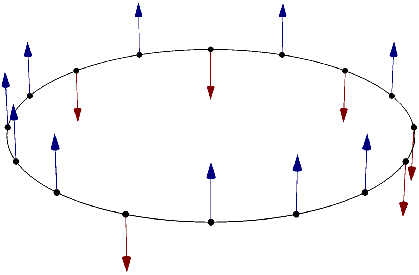
\includegraphics[width=0.8\textwidth]{Figures/ring.pdf}
    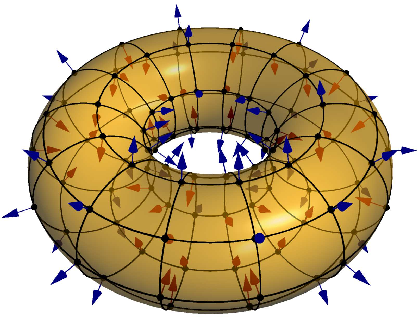
\includegraphics[width=0.8\textwidth]{Figures/torus.pdf}
    \caption{Visualization of periodic boundary conditions in 1-D (circle topology) and
    2-D (torus topology).}
    \label{fig:pbc}
\end{figure}

